
\subsection{Cross Sections as a function of \tkialpha } 

Figure~\ref{figure:xsec_alph} shows the differential cross section as a function of \tkialpha \ for interactions on the CH, C, H$_{2}$O, Fe, and Pb targets, respectively. 
%The data are represented by the black dots with error bars.  The expectation from the simulation (MnvGENIE) is given by the histograms and is broken down by the interaction process. 
\tkialpha \ is the angle that measures the direction of the transverse momentum imbalance between the incoming neutrino and the sum of the lepton and hadron momenta.  It is sensitive to the intranuclear momentum transfer that comes from nucleon correlations and FSI.  MINERvA has measured \tkialpha \ previously for interactions on scintillator in the LE run~\cite{MINERvA:2018hba}.  The uncertainties broken down by source for both the absolute cross sections and the cross section ratios as a function of \tkialpha\ can be found in Fig.~\ref{fig:xsec_err_alpha}.


% tki_alpha xsecs
\begin{figure}[h]  
	\centering
 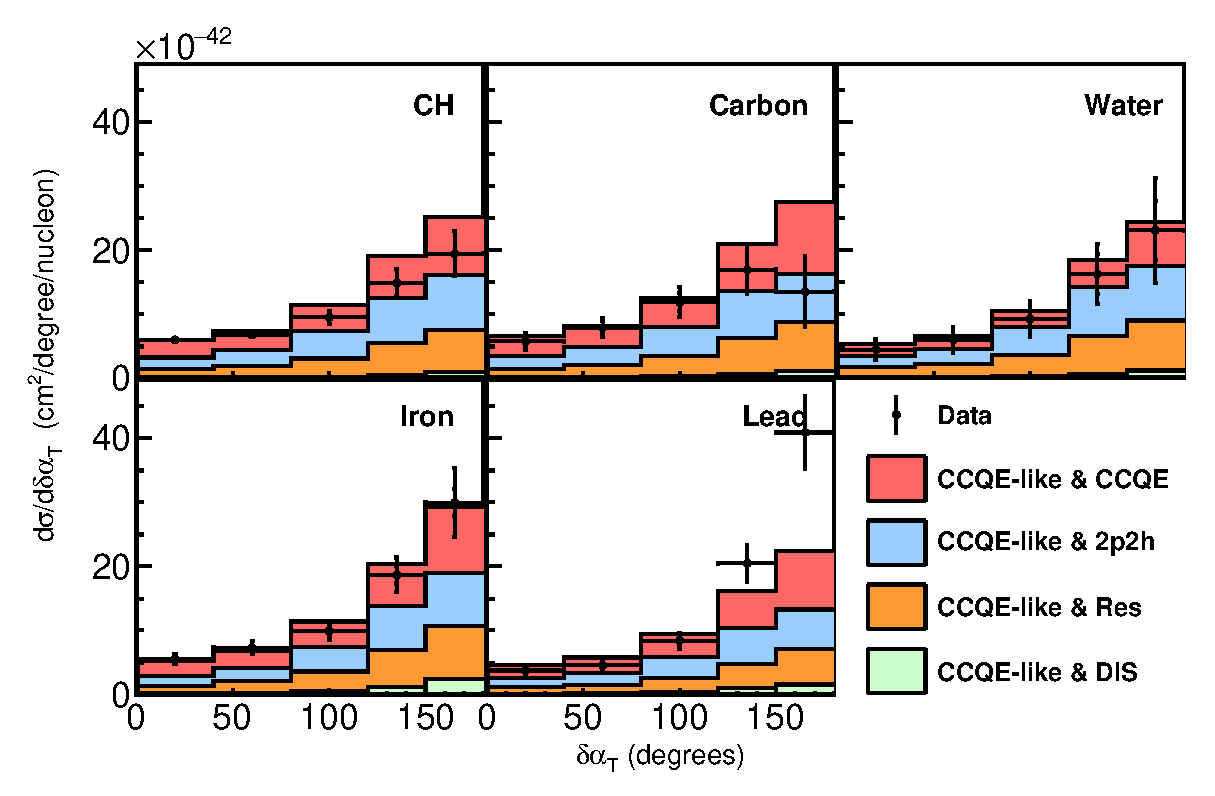
\includegraphics[width=\linewidth]{Figures/xsec_five_square/alpha.eps}
	\caption{The differential cross section as a function of \tkialpha \ for CH, C, H$_{2}$O, Fe, and Pb targets, along with the predictions for the different quasielastic-like signal processes.}
	\label{figure:xsec_alph}
\end{figure}

Here the largest discrepancies between the data and the simulation occur at large \tkialpha \ where the variable is most sensitive to FSI effects.  A larger \tkialpha \ indicates the proton losing momentum relative to the case without nuclear effects.  The simulation significantly overpredicts the cross section at high \tkialpha \ for the 
carbon and scintillator targets and underpredicts what is seen at high \tkialpha \ for lead.


The differential cross section as a function of \tkialpha \ for the different targets is shown in Fig.~\ref{fig:models_alphat}.  Also shown for comparison are results for a range of models. The observed comparisons are similar to what was seen for $\phi_{T}$ and \tkidelta :  NEUT predicts more events than seen in the data, particularly in regions where the FSI is expected to be large.  The hN versions of GENIE give predictions approaching NEUT in those high FSI regions at large \tkialpha \ for the larger targets.  The other generators do fairly well in simulating what is seen in the data although the MINERvA tune, NuWro SF and GENIE v3 G18\textunderscore 01a underpredict the data in Pb where the FSI is expected to be most pronounced.  The \chisq\ between the cross sections and the models can be found in Table~\ref{tab:dalphat}.

% comparisons to generators TKI alpha
\begin{figure}
    \centering
        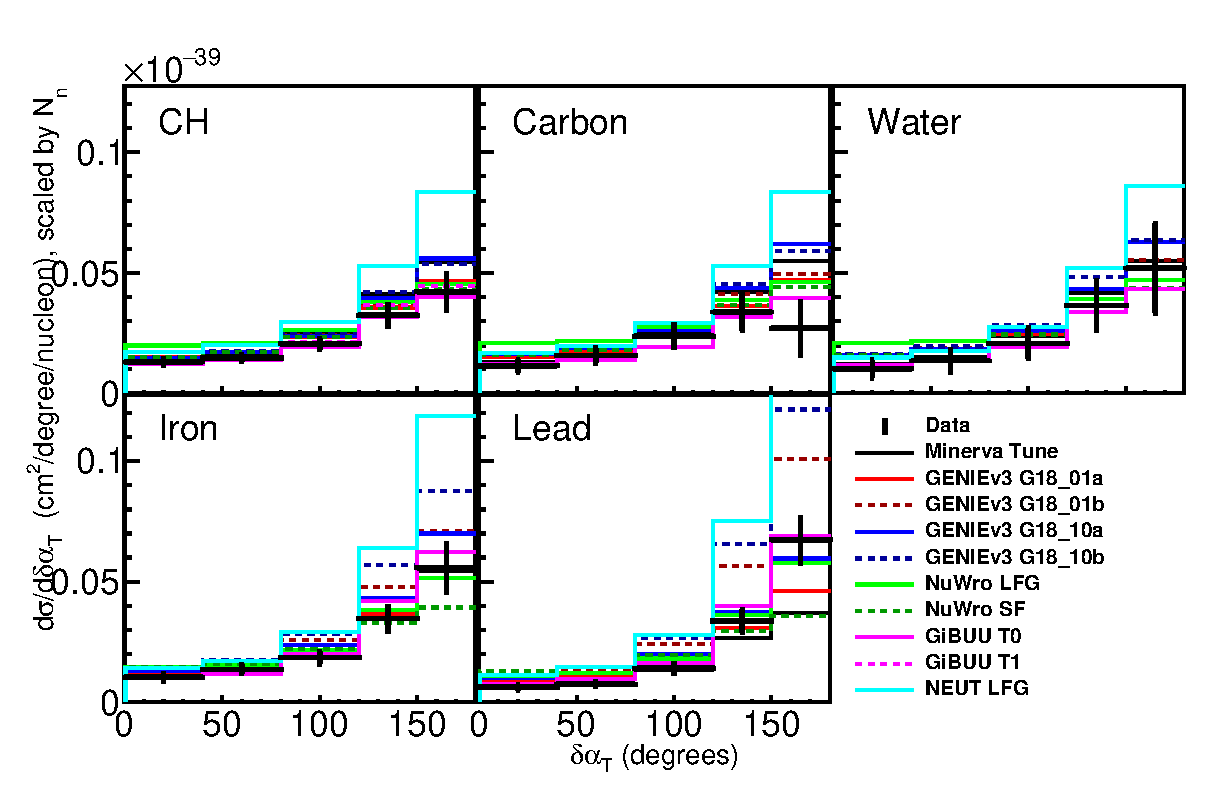
\includegraphics[width=\linewidth]{Figures/gencompare/alpha_5square.eps}
    \caption[\tkialpha \ cross-section comparison for multiple targets ]{Cross section measurements and predictions as a function of \tkialpha\ for different targets and for a selection of different generator and model choices.}
    \label{fig:models_alphat}
\end{figure}

The ratio of the differential cross section as a function of the \tkialpha \ for each nuclear target (C, H$_{2}$O, Fe, Pb) to that for scintillator is shown in Fig.~\ref{Figure:Gencompare_alpha_ratio}. The ratios show reasonable agreement between the data and the MINERvA tune except at high \tkialpha \ in Fe and Pb, where the model spread grows.  NEUT and the hN versions of GENIE predict a higher ratio where at large \tkialpha , where the FSI is greatest.  In the same region the hA versions of GENIE and NuWro predict a smaller ratio than seen in the data.  The \chisq\ between the cross section ratios and the models can be found in Table~\ref{tab:dalphat}.  

\begin{figure}
    \centering
        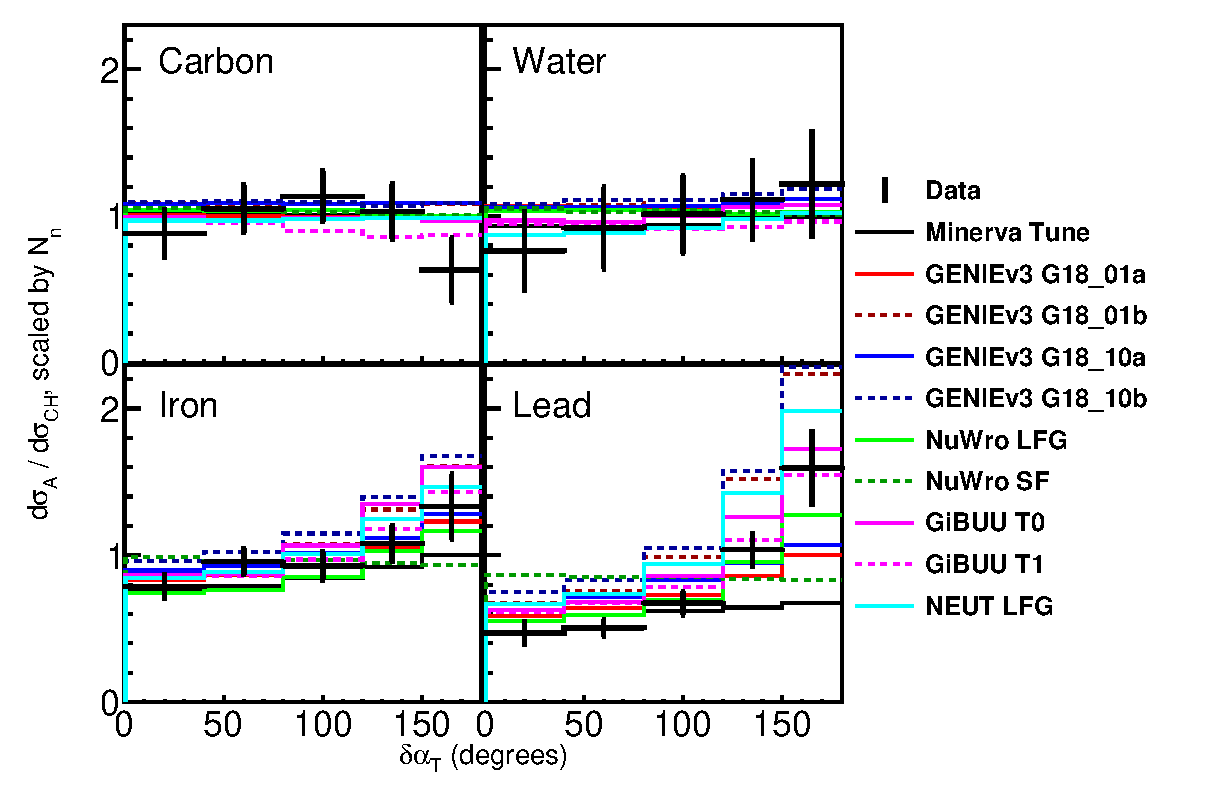
\includegraphics[width=\linewidth]{Figures/gencompare/alpha_4square.eps}
    \caption{Cross-section ratios as a function of \tkialpha\ for different generators and multiple targets.  Note that changes to the FSI model (GENIE ``a'' to ``b'')
     in GENIE change the cross section ratio at both intermediate and high \tkialpha\  more than changes to the 2p2h model (GiBUU T0 to GiBUU T1) or changes to the initial state (GENIE 1 to GENIE 10) or (NuWro LFG to NuWro SF). }
        \label{Figure:Gencompare_alpha_ratio}
\end{figure}

 